%Commandi utili ridefiniti

\newcommand{\COURSE}{Ingegneria del software}

\newcommand{\STUDENT}{Grigoras Valentin}
\newcommand{\MATRICOLA}{1099561}
\newcommand{\ANNO}{A.A 2018/2019}




% ----------------------- TODO ---------------------------

\documentclass[a4paper]{article}
\usepackage[utf8]{inputenc}
\usepackage[T1]{fontenc}

\usepackage[italian]{babel}

\usepackage{fancyhdr}
\usepackage{color}

\usepackage{lastpage}
\usepackage{listings}
\usepackage{tikz}

\usepackage{subfigure}
\usepackage{float}
\usepackage{hyperref}
\usepackage{tabularx}
\usepackage{color}
\usepackage{geometry}
\usepackage{fancybox}

\usepackage{utopia}
\usepackage{lipsum}
\usepackage{amstext}
\usepackage{xcolor}
\usepackage{listingsutf8}
\lstset{inputencoding=utf8/latin1}
\definecolor{blue}{HTML}{007af7}
\definecolor{red}{HTML}{920022}
\definecolor{grey}{HTML}{fdfcf8}
\definecolor{comment}{HTML}{1b9852}
\definecolor{strings}{HTML}{5f283e}

\definecolor{tipo}{RGB}{167, 63, 74}
\definecolor{variabile}{RGB}{32, 114, 154}

\lstset{language=Java,backgroundcolor=\color{grey}, commentstyle=\color{comment},identifierstyle  = \color{blue},extendedchars=true, frame=single,keepspaces=true, keywordstyle=\color{red},tabsize=3,showstringspaces=false,literate={é}{{\'{e}}}1, literate={è}{{\'{e}}}1 }


\input kvmacros

%Größe der Ränder setzen
\geometry{a4paper,left=3cm, right=3cm, top=3cm, bottom=3cm}

%Kopf- und Fußzeile
\pagestyle {fancy}
\fancyhead[L]{\COURSE}
\fancyhead[C]{}
\fancyhead[R]{\rightmark }

\fancyfoot[L]{}
\fancyfoot[C]{}
\fancyfoot[R]{Pagina \thepage /\pageref*{LastPage}}

%Formatierung der Überschrift, hier nichts ändern
\def\header#1#2#3#4{
\vspace*{\fill}
  \begin{center}
    { \Large Appunti Ingegneria del software #1}\\ \vspace{10pt}
    {(\ANNO #2)} \\  \vspace{10pt}
{\Large \STUDENT#3} \\  \vspace{10pt}
{\Large Matricola: \MATRICOLA #4} \\  \vspace{10pt}
  \end{center}
  \vspace*{\fill}
}


\begin{document}

\header{}{}{}{}

\pagebreak

	\renewcommand{\contentsname}{Contenuti}
	\renewcommand\tablename{new}
	\tableofcontents \pagebreak

\vspace{30pt}
\section{Indicare le differenze (natura, finalita, collocazione) che intercorrono tra le attivitaa di \textbf{verifica} e quelle di \textbf{validazione}} \pagebreak
\subsection{Fissando l'attenzione sulla definizione di "processo" associata allo standard ISO/IEC 12207, indicare come (secondo quali regole), quando (in quali fasi di progetto) e perché (attraverso quali attività) la vostra esperienza di progetto didattico ha visto attuato tale concetto.}

Un processo è un insieme di attività \textbf{correlate}(ovvero contiene solo attività che hanno a che fare con il progetto)  e \textbf{coese}(un insieme di cose è coeso se tutto ciò che c’è serve, ci deve essere e se non ci fosse mancherebbe, quindi non c'è nulla di superfluo) con l'obiettivo di rispondere ai bisogni in ingresso restituendo risposte (prodotto delle attività del processo) in uscita agendo secondo regole date consumando risorse nel farlo. Significa che un processo non è mai solo perché sopra di lui c’è un \textit{controllo} che sa come le cose stanno andando perché emette vincoli sul modo in cui il processo lavora misurando l'efficienza e l'efficacia.

L'efficienza si misura con l’efficienza produttiva. Guardo quindi il rapporto tra quantità di prodotto realizzato e risorse utilizzate.

L'efficacia invece si misura in base a quanti obiettivi interni (del fornitore) o esterni (gradimento del cliente) raggiungo.

L’insieme di efficienza ed efficacia si chiama economicità, ovvero raggiungo gli obiettivi se sono efficace consumando poche risorse.

L'ISO/IEC 12207 contiene una descrizione approfondita dei processi del ciclo di vita del software, ed è infatti il modello più noto e riferito, anche se ne esistono altri. Questo modello è ad alt livello, ed identifica i processi dello sviluppo software, ed ha una struttura modulare che permette, nel processo di specializzazione, di identificare le entità responsabili dei processi ed i prodotti dei processi.
Secondo questo modello si hanno processi (processes), che sono divisi in attività (activities) che, a loro volta, sono divisi in compiti (tasks). Così si ha una struttura modulare (perchè i processi si interfacciano), ma con una forte coesione (perchè i compiti sono chiusi). I processi descritti in ISO 12207  hanno lo scopo di eliminare tutti gli sprechi di tempo e risorse, eliminando le particolari attività per un progetto specifico.
Nel corso del progetto didattico, si è innanzitutto cercato di determinare i processi necessari allo sviluppo del prodotto attenendosi fedelmente allo standard ISO/IEC 12207. Si è poi passati alla definizione generica delle attività costituenti ogni processo per poi contestualizzarla e dettagliarla sempre più con il progredire del progetto. Si è dunque assicurati che all’istanziazione di ogni processo questo fosse normato e ben definito rispetto alle attività che lo compongono e alle sue pre e post condizioni. Da un punto di vista pratico, questo approccio ha permesso di lavorare secondo una migliore suddivisione in task, migliorarndo progressivamente la qualità dei processi una volta concluse le relative attività e verificati i relativi prodotti.  \pagebreak
\subsection{Fornire una definizione del formalismo noto come "diagramma di Gantt", discuterne concisamentele finalità e modalità d'uso, l'efficacia e i punti deboli eventualmente rilevati nell'esperienza delprogetto didattico}
Il diagramma di Gantt, usato principalmente nelle attività di project management, è uno strumento che serve a pianificare un insieme di attività in un certo periodo di tempo. È costituito da 2 assi. Sull'asse orizzontale si indica il tempo totale del progetto, suddiviso in fasi incrementali (ad esempio, giorni, settimane, mesi), mentre sul asse verticale ci sono le attività da svolgere avente un tempo d’inizio e un tempo di fine, ma non la quantità di lavoro in termini di ore. 

Le barre orizzontali di lunghezza variabile rappresentano le sequenze, la durata e l'arco temporale di ogni singola attività del progetto. Le attività da svolgere possono essere  sovrapposte durante il medesimo arco temporale ad indicare la possibilità dello svolgimento in parallelo di alcune delle attività, oppure dipendenti se un’attività finisce prima che inizi la successiva attività.

Una linea verticale è utilizzata per indicare la data di riferimento. 

Il diagramma di gantt permette quindi di visualizzare chiaramente il flusso di lavoro mostrando la data di inizio e di fine di una determinata attività, consentendo un uso intelligente ed efficace delle risorse.
  \pagebreak
\section{Dare una definizione ben fondata del concetto di "architettura software". In relazione a tale concetto, dare una definizione ai termini "framework" e "design pattern" spiegando come questi si integrino fra loro E all'interno di una architettura. }

\textbf{Un'architettura software} è un insieme di elementi architetturali, utilizzati secondo una particolare forma(intesa come organizzazione e strutturazione) insieme a una giustificazione logica che coglie la motivazione per la scelta degli elementi e della forma. Per  \textbf{forma} si intende la divisione di tale sistema in componenti, nella disposizione di essi e nei modi in cui tali componenti comunicano tra loro. \textbf{La giustificazione logica} ha lo scopo di rendere esplicite le motivazioni per la scelta degli elementi e della forma – in particolare, con riferimento al modo in cui questa scelta consente di soddisfare i requisiti/interessi del sistema.
\textbf{Lo scopo dell'architettura software} è di facilitare lo sviluppo, la distribuzione, il funzionamento e la manutenzione del sistema software in esso contenuto, quindi di supportare il ciclo di vita del sistema. \\

\textbf{Un pattern software} è una soluzione provata e ampiamente applicabile a un particolare problema di progettazione che è descritta in una forma standard, in modo che possa essere facilmente condivisa e riusata. 

Un \textbf{design pattern} è la descrizione di oggetti e classi che comunicano tra di loro, personalizzati per risolvere un problema generale di progettazione in un contesto particolare. I design pattern sono spesso utili nel descrivere le connessioni tra elementi architetturali indicando un approccio uniforme nella loro realizzazione.
\textbf{I benefici dei design pattern} soprattutto dal punto di vista dell’architettura del software sono la riduzione del rischio, sulla base di soluzioni provate e ben comprese e un maggior incremento della produttività, della standardizzazione e della qualità. \\

Con la parola \textbf{framework} intendiamo una micro architettura che mette a disposizione tipi estendibili nell'ambito di uno specifico dominio. Nell'archietttura software un framework è una parte di software riutilizzabile ed estendibile.  \pagebreak
\subsection{Fornire una definizione del concetto di \textit{qualità}, applicabile al dominio dell'ingegneria del software. Discutere concisamente quali attivita' il proprio gruppo di progetto didattico abbia svolto nella direzione di tale definizione, indicando allo stato attuale di progetto  i migliori e i peggiori risultati ottenuti, offrendo una spiegazione dell'esito}

La \textbf{qualità di un oggetto} è una caratteristica che si basa su proprieta' misurabili del prodotto, cioè su quantità confrontabili con degli standard prefissati; nel caso del software, però, queste proprietà \textit{misurabili} sono più difficili da quantificare rispetto agli oggetti fisici. Tuttavia, anche per il software sono state standardizzate delle metriche che riguardano la complessita' ciclomatica, la coesione, il numero di function-points, il numero di righe di codice.

Il \textbf{controllo della qualità} viene fatto attraverso l'attività di software quality assurance che si compone di un’attività di gestione della qualità, revisioni tecniche formali svolte durante il processo, una strategia di collaudi su più livelli, una gestione della documentazione e delle modifiche, una procedura che garantisca la conformità allo standard dello sviluppo, e infine meccanismi di misurazione e stesura dei resoconti.

La \textbf{qualità del software} è il rispetto dei requisiti funzionali e prestazionali enunciati esplicitamente, la conformità a standard di sviluppo esplicitamente documentati e le caratteristiche implicite che ci si aspetta da un prodotto software realizzato professionalmente.

Da questa definizione emergono tre punti fondamentali per lo svolgimento dell'attività di SQA:
\begin{enumerate}
 \item i requisiti sono alla base delle misurazioni della qualità; la non conformità ai requisiti implica mancanza di qualità;
\item gli standard specificati definiscono i criteri da seguire durante lo sviluppo del software;
\item anche i requisiti impliciti devono essere tenuti in cosiderazione; un software che rispetta i requisiti
espliciti ma non quelli impliciti è spesso un software di scarsa qualità.
\end{enumerate}

Durante il corso del progetto, la qualità è stata perseguita definendo obiettivi ad essalegati, monitorati mediante misurazioni metriche pertinenti e raggiunti tramite apposite strategie. L'attività di quality assurance ha accertato che il grado di conseguimento degli obiettivi fosse in linea con quanto previsto, e l'impianto amministrativo, le procedure e gli strumenti automatici dedicati hanno concretizzato la politica di qualità stabilita dal gruppo. Sotto uno sguardo critico, lo svolgimento di tali attività è stato tuttavia superficiale e lacunico, producendo falle nel sistema di attuazione della qualità cui ha conseguito il mancato raggiungimentodi alcuni obiettivi proposti. Tale problema si sarebbe probabilmente potuto mitigare con una migliore attività di formazione del personale.  \pagebreak
\subsection{Spiegare concisamente (dunque a livello di sostanza) la differenza tra il modello di sviluppo iterativo e quello incrementale. Alla luce dell'esperienza acquisita nel progetto didattico, indicare spiegando a posteriori, quale dei due sarebbe stato più adatto al caso}

Nello \textbf{sviluppo iterativo} lo sviluppo del software è organizzato in una serie di mini-progetti brevi, di lunghezza fissa (ad es., 2-4 settimane) chiamati iterazioni. \textbf{Un'iterazione} consiste nella ripetizione di un dato insieme di attività fino a che queste non convergono ad un dato obiettivo, rimandando alla fine l’integrazione delle componenti sviluppate. Ciascuna iterazione comprende le proprie attività di analisi dei requisiti, analisi, progettazione, implementazione, verifica.  Il sistema cresce in modo incrementale da un'iterazione alla successiva, adattandosi ai requisiti, in modo evolutivo, sulla base del feedback delle iterazioni precedenti. Il risultato di ciascuna iterazione è normalmente un sistema incompleto, che converge verso un sistema completo dopo varie iterazioni.
L'articolazione di un progetto iterativo è guidata non da una rigida seguenza di fasi predefinite, ma da una gestione sistematica dei rischi di progetto, per arrivare alla loro progressiva diminuzione.


Nel \textbf{modello incrementale} i cicli non sono più iterazioni ma incrementi. Il termine \textbf{incremento} designa un'aggiunta o un'avanzamento. Ogni incremento attraversa tutte le fasi del modello sequenziale, dall'analisi alla verfica.

Il modello prevede rilasci multipli realizzando un incremento di funzionalità e avvicinandosi sempre più alle attese. Un grande vantaggio è che le funzionalità più importanti vengono trattate per prime; così facendo, queste vengono verficate più volte (dato che ogni ciclo prevede la verfica del software). 

Ogni incremento ha il vantaggio di ridurre il rischio di fallimento, con un approccio più realistico e predisposto ai cambiamenti. Difatti, mentre il modello sequenziale segue un approccio predittivo (cioè basato su piani che devono essere rispettati), il modello incrementale segue un approccio adattativo, dove la realtà è considerata imprevedibile. 

Un grande vantaggio offerto è rappresentato dal fatto che le funzionalità critiche vengono trattate per prime, subendo così una ripetuta verifica.
Valutando il progetto a posteriori, il modello più adatto al caso è probabilmente quello incrementale, che grazie al suo focus sulla verifica delle funzionalità critiche dà maggiori garanzia di corretta implementazione delle stesse. La scelta del modello incrementale permette inoltre di ripetere più e più volte varie fasi del progetto, consentendo ad un team inesperto di impratichirsi maggiormente con le attività ad esse legate.  \pagebreak
\section{Fornire una definzione dei concetti di \textbf{milestone} e \textbf{baseline}, indicando come ciascuno di essi sia da utilizzare all'interno delle attività di progetto.}
Una \textbf{baseline} è un punto di avanzamento consolidato, fissato strategicamente in risposta a qualche discussione con gli stakeholders. Una baseline è fatta di parti chiamati CI (configuration item ) utili al raggiungimento di obiettivi strategici in un tempo breve. Le parti di cui è fatta una baseline (le quali hanno un numero di versioni “as many as needed”), esistono perchè assolvono un obiettivo.
Ogni punto di avanzamento viene fissato precedentemente in modo strategico dalla best practice, ma il numero di baseline non è deciso a priori:  solo gli obiettivi sono decisi a priori.
Una baseline si costruisce con la configurazione e si mantiene con il versionamento.

Una \textbf{milestone} definisce un traguardo da raggiungere, pianificato e misurabile. Un traguardo è la fine di una fase di progetto in corrispondenza della quale può essere rivisto l'avanzamento del lavoro. Ogni milestone deve essere documentata da un breve report che riassume lo stato del software che si sta sviluppando e ne verifica la completezza rispetto a quanto specificato nel piano di progetto.
Questo report chiamato output formale della milestone viene poi presentato al responsabile.
Durante le fasi critiche del progetto come per esempio nella fase di progettazione, vengono fatte delle consegne al cliente che attestastano lo stato di avanzamento del prodotto. Le consegne in genere sono delle milestone, ma le milestone non sempre sono delle consegne, in quanto una milestone può rappresentare dei risultati interni usati dal responsabile del progetto per verificare i progressi interni; questo tipo di milestone non vengono consegnati al cliente. Una milestone è concretizzata da almeno una baseline e dev'essere specifica, raggiungibile, misurabile (per quantità di impegno necessario), traducibile in compiti assegnabili e dimostrabile agli stakeholder. Il numero di milestone lo decide il fornitore.

Le milestone, concretizzate da una o più baseline, sono dunque elementi da pianificare con cura in quanto rappresentano stati d’avanzamento fondamentali per il progetto e riferimenti per il confronto fra stakeholders. Le baseline sono invece legate strettamente al controllo di configurazione ed in particolare al versionamento, che tramite repository assicura una versione comune (e auspicabilmente misurata e testata) del codice su cui basare i successivi incrementi.  \pagebreak
\subsection{Descrivere la tecnica di classificazione e tracciamento dei "requisiti" adottata nel proprio progetto didattico e discuterne l'efficacia e i limiti eventualmente riscontrati.}

Un \textbf{requisito} è una descrizione astratta di come dovrebbe essere il comportamento del sistema o di alcuni suoi vincoli. Il documento analisi dei requisiti ha lo scopo di elencare e descrivere in modo formale l'insieme dei requisiti.

Gestire la \textbf{tracciabilità dei requisiti} nel flusso di progetto è la chiave per una progettazione più efficiente e più efficace.  Più efficiente perché consente di velocizzare e gestire in modo ottimale tutte le varianti di progetto, in ogni sua fase. Inoltre è più efficace, perché permette di mantenere il progetto fedele alle specifiche iniziali, che corrispondono ai requisiti desiderati del committente, anche se lungo il flusso emergono vincoli non previsti inizialmente.

L'attività di \textbf{classificazione e tracciamento dei requisiti} si è divisa in più fasi. Inanzitutto si è scelto il modello per il ciclo di vita del software più idoneo al nostro progetto. Si è scelto un approccio incrementale perchè i requisiti non erano sufficientemente chiari nella prima fase del progetto. Questo ci è permesso, in seguito alla discussione con il proponente, di redigere i requisiti obbligatori e quelli desiderabili, anche se col avanzare del tempo si è dovuto rinegoziare con il proponente cambiando alcuni requisiti.

Per la \textbf{scoperta dei requisiti} sono state utilizzate alcune tecniche, quali:
\begin{itemize}
\item identificazione dei \textbf{casi d'uso}, che ci è permesso di analizzare le modalità di utilizzo del sistema.
\item \textbf{interviste} con il proponente;
\item \textbf{brainstorming}, grazie alla quale sono state raccolte e organizzate le idee di ogni componente del gruppo su come il sisteme deve comportarsi;
\end{itemize}

La tecnica utilizzata per la traccibilità dei requisiti è stata quella di assegnare un identificatore univoco a ciascun requisito rigorosamente documentato nel documento norme di progetto. L'identificatore ha la seguente forma:
\begin{center}
\textbf{R[Priorità][Tipo][Codice]}
\end{center}
Ogni requisito ha una sua priorità che può essere di tre livelli: obbigatorio (0), desiderabile (1) e opzionale (2).

Ogni requisito si differenzia in 4 diverse tipologie: funzionali (F), prestazionali (P), qualitativi(Q).

Apposite tabelle hanno poi permesso di associare ogni requisito alle proprie fonti e ai casi d’uso corrispondenti. 

Con queste premesse, non sono emersi particolari problemi nel tracciamento dei requisiti in sé, quanto più nel livello di dettaglio degli stessi che talvolta rendeva ambigua la conferma del loro soddisfacimento.  \pagebreak
\section{Discutere la differenza tra le attività di "versionamento" e "configurazione" come vengono applicate all'ambito dello sviluppo sw}
Una \textbf{configurazione} indica le parti di un prodotto software e come esse vengono messe insieme. Le attività di configurazione vanno pianificate e la loro gestione va automatizzata. Esse servono a mettere in sicurezza la baseline, prevenire sovrascritture e permettere il ritorno alle versioni precedenti.
Nell'ambito dello sviluppo software la gestione della configurazione si occupa di 4 attività:
\begin{itemize}
	\item \textbf{Identificazione di configurazione} ovvero dividere il prodotto in configuration item;
	\item \textbf{Controllo di baseline} ovvero definire le baseline che portano ad una milestone garantendone riproducibilità, tracciabilità, analisi e confronto;
	\item \textbf{Gestione delle modifiche} ovvero le richieste di modifiche di utenti, sviluppatore e competizioni sono sottoposte ad analisi, decisione, realizzazione e verifica, e le modifiche devono essere tracciabili e ripristinabili;
\item \textbf{Controllo di versione} cioè VERSIONAMENTO;
	\end{itemize}
Una \textbf{versione} è un'istanza di un determinato configuration item, diversa dalla precedente. Il versionamento consente tramite repository di contenere tutti i configuration item di ogni baseline e la loro storia.
Dunque il versionamento si occupa dei CI di una baseline, e di come vengono identificati e gestiti, mentre la configurazione si occupa anche dell'organizzazione del prodotto, oltre che del versionamento, e dell'integrazione delle parti nel prodotto finale.  \pagebreak
\section{Presentare due metriche significative per la misurazione di qualità della progettazione software e del codice( quindi almeno una metrica per ciascun oggetto). Giustificare la scelta in base all'esperienza maturata nell'ambito del proprio progetto didattico. Discuter brevemente l'esito osservato del'eventuale uso pratico di tali metriche}

Lo IEEE definisce una metriche come una misura quantitativa del grado in cui un sistema, componente o processo possiede un certo attributo.
Una metrica per la progettazione software è \textbf{l'instabilità}, che indica il rapporto tra coesione e accoppiamento di una componente. Una \textbf{coesione} indica quanto le parti interne della componente siano legate tra loro. Una coesione alta è indice di una componente modulare, compatta e specializzata. \textbf{L'accoppiamento} indica invece quante dipendenze la componente ha con l'esterno. Maggiore è l'accoppiamento, minore è la mantenibilità e la modularità della componente. Un valore basso di instabilità indica una forte coesione e uno scarso accoppiamento, mentre un valore alto è sintomo di un accoppiamento troppo forte. L'obiettivo di tale metrica è di rendere il software più modulare è manutenibile possibile.

Una metrica per il codice è la\textbf{ complessità ciclomatica}, che indica il numero di cammini indipendenti che l'esecuzione di un metodo può intraprendere. Un valore alto è sintomo di un metodo troppo complesso, scarsamente modulare e manutenibile. 

Nel progetto didattico è stata utilizzata questa metrica che ci ha permesso di rendere i metodi più modulari e facili da testare.  \pagebreak
\section{OOP PRINCIPLES REVISITED}

La OOP è un paradigma di programmazione basato sul concetto di oggetto. Questo oggetto contiene dati e/o metodi/procedure. La caratteristica maggiore è che il paradigma oop le procedure degli oggetti possono accedere ai dati.


\subsection{Oggetto}

\begin{itemize}
\item è un istanza della classe;
\item definizione secondo Grady Booch: "un oggetto rappresenta un articolo (item), un'unità o un'entità individuale, identificabile, reale o astratta che sia, con un ruolo ben definito nel dominio del problema e un confine altrettanto ben stabilito";

Generalmente un oggetto è caratterizzato da uno stato, da un comportamento e da un'identità, come bene simboleggiato da questa illustrazione tratta, come quelle che seguono, da G. Booch, Object-oriented Analysis and Design:

\begin{figure}[H]
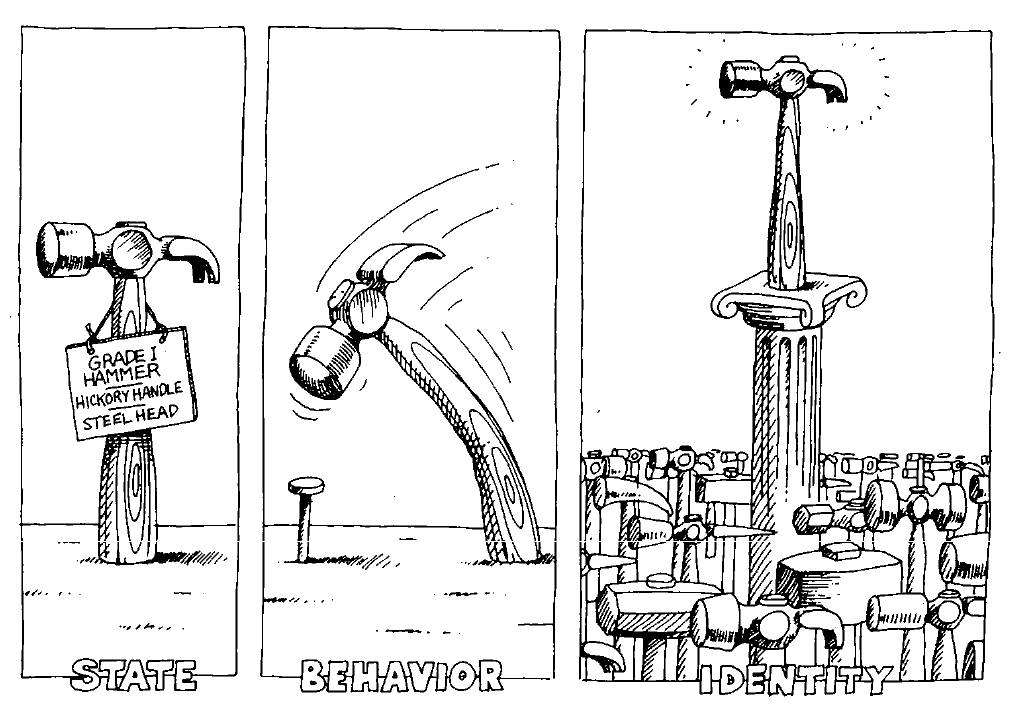
\includegraphics[scale=0.4]{images/oggetto}
\caption{Definizione di oggetto  \label{fig:oggetto}}
\end{figure}
\end{itemize} 

\subsubsection{Elementi fondamentali di un oggetto}

“Un oggetto possiede stato, comportamento e identità; la struttura e il comportamento di oggetti simili sono definiti nella loro classe comune; i termini di istanza e oggetto sono intercambiabili.” [Grady Booch].

\paragraph{Stato}

Gli oggetti, tipicamente, non vengono creati per permanere in un determinato stato; al contrario, durante il loro ciclo di vita transitano in una serie di fasi.

Tipi di stato:
\begin{itemize}
\item \textbf{oggetto con un insieme finito di stati}: per esempio l'oggetto lampadina ha 2 stati: acceso e spento. Un altro esempio è una lampadina evoluta con un numero ben definito di diverse intensità di luce, quindi avrò gli stati spenta, accesa intensità 1, accesa intensità 2, ..., accesa intensità max;

\item \textbf{oggetto con un numero di stati non numerabili}: per esempio un sistema di illuminazione delle stanze la cui funzione sia accendere/spegnere i vari faretti in funzione del numero di persone presenti nelle stanze. Sebbene questo numero sia delimitato (il numero massimo di persone stipabili all'interno della stanza), non è conveniente indicare i vari stati dell'oggetto (una persona, due persone, tre persone, …);

\item \textbf{oggetto con stati teoricamente infinito}: per esempio, si consideri un'estensione del sistema precedente, in cui la decisione di accendere e/o spegnere l'illuminazione dipenda anche dal valore dell'intensità luminosa segnalata da un apposito oggetto (sensore). In questo caso, il dominio dei valori dei dati forniti sarebbe teoricamente infinito.

\end{itemize}

Lo stato di un oggetto è molto importante poiché ne influenza il comportamento futuro. Gli oggetti, almeno loro, hanno una certa memoria storica. Tipicamente, sottoponendo opportuni stimoli a un oggetto (invocazione dei metodi, o invio di messaggi se si preferisce), questo tende a reagire, nella maggior parte dei casi, in funzione del suo stato interno.

\textbf{Esempio 1}: se una sua istanza si trova nello stato di accesa e ne viene richiesta nuovamente l'accensione (turnOn()), nulla accade.

\textbf{Esempio 2}: se si preme il tasto di play senza aver inserito un CD, nulla accade (viene generata un'eccezione), mentre la pressione dello stesso tasto, con CD inserito, avvia il suono della musica.

Lo stato di un oggetto è un concetto dinamico e, in un preciso istante di tempo, è dato dal valore di tutti i suoi attributi e dalle relazioni instaurate con altri oggetti (che alla fine sono ancora particolari valori, indirizzi di memoria, attribuiti a specifici attributi).

È molto importante nascondere quando possibile lo stato di un oggetto al resto del mondo. Sicuramente deve esserne sempre nascosta l'implementazione (principio \textit{dell'information hiding}) e quando possibile anche lo stato stesso (minimizzare l'accoppiamento di tipo).

\paragraph{Comportamento}

Una volta studiato e formalizzato lo stato di un oggetto si è effettuato un passo in avanti nel processo di astrazione.

Tipicamente un oggetto interagisce con altri scambiando messaggi, ossia rispondendo agli stimoli provenienti da altri oggetti (richiesta di un servizio) e, a sua volta, inviandoli ad altri al fine di ottenere la fornitura di "sottoservizi" necessari per l'espletamento(completamento) del proprio. Quindi, il comportamento di un oggetto è costituito dalle sue operazioni visibili e verificabili dall'esterno.

"Il comportamento stabilisce come un oggetto agisce e reagisce, in termini di cambiamento del proprio stato e del transito dei messaggi." [Booch].

\textbf{Un'operazione} è una qualsiasi azione che un oggetto è in grado di richiedere a un altro al fine di ottenere la reazione desiderata.

È evidente che la relazione esistente tra stato di un oggetto e comportamento è di mutua dipendenza: è possibile considerare "lo stato di un oggetto, in un certo istante di tempo, come l'accumulazione dei risultati prodotti dal relativo comportamento", il quale, a sua volta, dipende dallo stato in cui si trovava l'oggetto all'atto dell'esecuzione del "comportamento".

\paragraph{Identità}

 \noindent L'identità di un oggetto è la caratteristica che lo contraddistingue da tutti gli altri. Spesso ciò è dato da un valore univoco. Per esempio un oggetto ContoCorrente è identificato dal relativo codice, da una persona, dal codice fiscale, e così via.

 \subsection{Classe}
 \begin{itemize}
\item è un prototipo che descrive com'è fatto una certa tipologia di oggetti.
 \end{itemize}
 
 \subsection{Tempo di implementazione vs tempo di esecuzione}
  \begin{figure}[H]
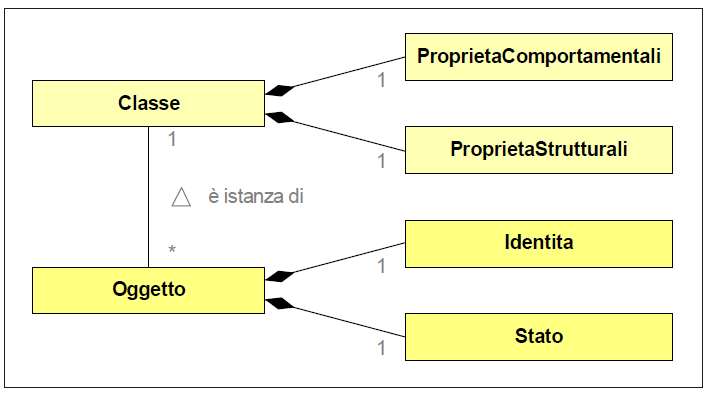
\includegraphics[scale=0.7]{images/esecuzioneVSimplementazione}
\caption{\textit{In questo (meta) modello sono distinte più nettamente le caratteristiche a tempo di implementazione (Classe, ProprietàComportamentali e ProprietàStrutturali) da quelle a tempo di esecuzione (Oggetto, Identità e Stato). \textbf{Le proprietà comportamentali} rappresentano l'insieme dei metodi esposti da una classe e quindi invocabili da parte di oggetti istanze di altre classi, mentre quelle \textbf{strutturali} rappresentano l'insieme degli attributi. Per quanto concerne la notazione, per il momento si consideri il diamante pieno (relazione di composizione) come una relazione strutturale molto forte tra due entità, di cui le istanze della classe con il diamante rappresentano il concetto generale costituito dalle istanze delle altre classi associate.}\label{fig:ered0}}
\end{figure}

\subsection{Principi cardini della OOP}

\subsubsection{Incapsulamento (information hiding)}
L'incapsulamento è il meccanismo che rende possibile il famoso principio dell'information hiding (nascondere le informazioni). Con tale termine ci si riferisce alla capacità degli oggetti di mostrare al mondo esterno, la propria organizzazione in termini di struttura e logica interna.

Una delle motivazioni alla base \textbf{dell'information hiding} è data dalla necessità di creare uno strato di separazione tra gli oggetti clienti e quelli fornitori. In altre parole è necessario separare l'interfaccia propria di un oggetto dalla sua implementazione interna. In sostanza l'interfaccia (anche se implicita) rappresenta il contratto stipulato tra gli oggetti client e quelli server. Ciò è vantaggioso al fine di aumentare il riutilizzo del codice e di limitare gli effetti generati dalla variazione della struttura di un oggetto.

In genere \textbf{l'incapsulamento standard} prevede che le classi non abbiano alcuna conoscenza della struttura interna delle altre, e in particolare di quelle di cui possiedono un riferimento, con la sola eccezione della firma dei metodi esposti nella relativa interfaccia. Ciò permette a ogni classe di modificare, aggiungere, rimuovere parte del proprio comportamento e della propria struttura interna senza generare alcun effetto sulle restanti classi.

Questo è vero fintantoché le variazioni non abbiano come dominio metodi appartenenti all'interfaccia della classe: è sufficiente anche la variazione di un solo parametro della firma di un metodo dell'interfaccia per rendere necessaria la modifica delle classi client.

Il principio dell'incapsulamento standard, in Object Oriented, si realizza rendendo privata la struttura interna della classe. Chiaramente una classe con tutti i metodi e gli attributi privati sarebbe di ben poco utilizzo.

Ciò che si desidera è, in definitiva, conferire una visibilità privata a quanta più parte di struttura e comportamento possibile (soprattutto agli attributi), limitandosi a esporre specifici metodi.
\paragraph{Difetti dell'incapsulamento}

Il nascondere il più possibile l'organizzazione della struttura delle classi, di fatto, limita o addirittura inibisce l'ereditarietà. Metodi e attributi privati non sono ereditati automaticamente, o meglio, sono ancora ereditati ma non accessibili, e quindi ridefinibili, dalla classe ereditante. In estrema sintesi si può asserire che la privacy non aiuta l'ereditarietà.

    \begin{itemize}
    \item Esempio di incapsulamento [Java] :
    \begin{lstlisting}
public class cubo
{
    // Dichiarazione delle proprieta: si noti che sono definite tutte private.
    private int lunghezza;
    private int larghezza;
    private int altezza;
    // Metodi "Mutator" per la modifica delle proprieta
    public void setLunghezza(int lun)
    {
        lunghezza = lun;
    }
    public void setLarghezza(int lar)
    {
        larghezza = lar;
    }
    public void setAltezza(int alt)
    {
        altezza = alt;
    }
    // Metodi "Accessor" per ricavare i valori delle proprieta
    public int getLunghezza()
    {
        return lunghezza;
    }
    public int getLarghezza()
    {
        return larghezza;
    }
    public int getAltezza()
    {
        return altezza;
    }
    // Metodo pubblico che visualizza il volume del cubo, usando le proprieta
    // interne della classe
    public void visualizzaVolume()
    {
        System.out.println(lunghezza * larghezza * altezza);
    }
}    \end{lstlisting}
     \end{itemize}


\subsubsection{Ereditarietà}

Si tratta di un meccanismo attraverso il quale un'entità più specifica incorpora struttura e comportamento definiti da entità più generali. Questo significa che la sottoclasse possiede tutti i campi e metodi della superclasse. Il fine cui si dovrebbe tendere attraverso l'utilizzo dell'ereditarietà è il "riutilizzo del tipo" perchè non c'è bisogno di ridescrivere quanto viene ereditato. Viceversa, le modifiche apportate alla sottoclasse sono limitate solo ad essa e non si applicano alla superclasse.

È possibile pensare all'ereditarietà come a un meccanismo in grado di prendere un elemento di partenza, clonarlo e di modificare e/o aggiungervi struttura e comportamento ulteriori.

\begin{figure}[H]
\includegraphics[scale=0.8]{images/ereditarietàUML}
\caption{\textit{La relazione di generalizzazione tra due classi è mostrata in UML attraverso una freccia collegante l'elemento figlio al proprio genitore, con un triangolo vuoto posto in prossimità di quest'ultimo.} \label{fig:oggetto}}
\end{figure}

\paragraph{Difetti}
\begin{itemize}
\item l’ereditarietà presenta punti di contrasto con il principio dell’incapsulamento: la classe antenata deve esporre propri dettagli interni alla classe ereditante, quindi modifiche alle classi antenate tendono a ripercuotersi su quelle discendenti.
\end{itemize}

\paragraph{Pregi}
\begin{itemize}
\item riutilizzo del codice, perchè il comportamento comune è definito una sla volta nella classe madre e riutilizzato nelle classi discendenti;
\item semplificazione della modellazione di sistemi reali;
\item utilizzo del polimorfismo perchè permette di dichiarare per una stessa operazione (metodo) definita in una classe antenata, diverse implementazioni ognuna localizzata in una delle classi discendenti;
\end{itemize}

\paragraph{Principio della sostituibilità}
Un’istanza di una classe discendente può sempre essere utilizzata in ogni posto ove è prevista un’istanza di una classe antenata.

\paragraph{Applicazione parziale del pattern Command}

\begin{figure}[H]
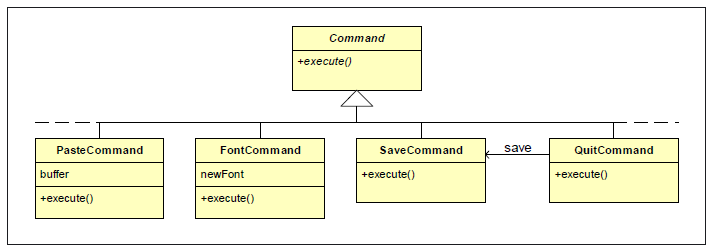
\includegraphics[scale=0.8]{images/commandEreditarita}
\caption{\textit{Gang Of Four (BIB04)} \label{fig:ered1}}
\end{figure}
In questo modello si è voluto mostrare un utilizzo più operativo della relazione di eredità. Come si può notare è possibile definire una classe generica Commanddotata di un metodo astratto execute()e quindi tutta una serie di specializzazioni atte a definire il comportamento del metodo in funzione delle responsabilità dello specifico comando. Per esempio, nella classe PasteCommand, il metodo execute() si occupa di copiare quanto presente nel buffer nell’area selezionata; nella classe QuitCommand, il metodo ha l’incarico di terminare l’esecuzione del programma (eventualmente chiedendo conferma) e, nel caso in cui vi siano cambiamenti non ancora memorizzati, ha l’ulteriore responsabilità di richiedere se salvare o meno i cambiamenti prima di terminare l’esecuzione.


\paragraph{Quando non applicare l'ereditarità}
\begin{itemize}
\item qualora in una struttura gerarchica un oggetto possa “trasmutare”, evidentemente l’applicazione della relazione di estensione è inappropriata e quindi è opportuno ricorre alla composizione;
\item ogniqualvolta in una struttura gerarchica un oggetto possa appartenere a più “tipi”, nuovamente non è opportuno utilizzare la relazione di generalizzazione.
\end{itemize}

\begin{figure}[H]
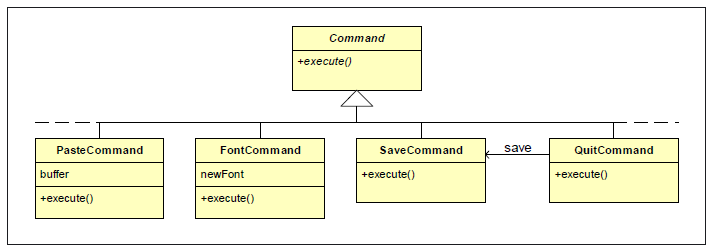
\includegraphics[scale=0.8]{images/commandEreditarita}
\caption{\textit{Esempio di errato utilizzo della relazione di ereditarietà. Da notare che con il termine di sviluppatore si intende far riferimento ai diversi ruoli implicati nella costruzione di sistemi (architetti, programmatori, tester, ecc.)} \label{fig:ered2}}
\end{figure}

È possibile identificare una serie di oggetti che esibiscono segmenti comuni di comportamento e/o struttura (per esempio la classe Persona) al quale ognuno aggiunge ulteriori specializzazioni (Cliente, Manager, Contabile, ecc.).

Cosa accade se un Commerciale, a un certo punto del suo ciclo di vita decide di diventare uno Sviluppatore? sarebbe necessario dar luogo a un’altra istanza, questa volta di tipo Sviluppatore, e quindi avere due oggetti diversi relativi allo stesso individuo con due identificatori distinti, con tutti i problemi derivanti. Ancora, cosa succederebbe se alcuni sviluppatori (per esempio Antonio Rotondi, Roberto Virgili), fossero così eccelsi da svolgere anche funzioni di Direttore? Queste due semplici domande sono sufficienti a dimostrare tutti i limiti dell’utilizzo della relazione di generalizzazione in contesti come questo.

\begin{figure}[H]
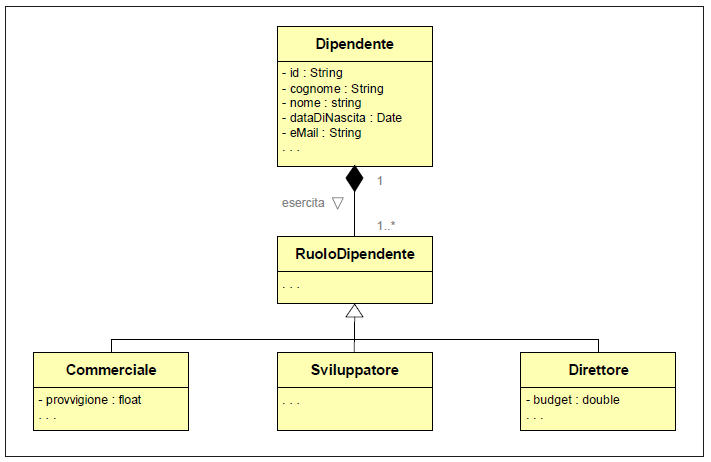
\includegraphics[scale=0.8]{images/ereditarietaOk}
\caption{\textit{Rappresentazione dei ruoli attraverso la relazione di composizione. Da notare che la classe RuoloDipendente non è strettamente necessaria} \label{fig:ered5}}
\end{figure}
\subsubsection{Polimorfismo}

Polimorfismo deriva dalle parole greche polys (= molto) e morphé (=forma): significa quindi “molte forme”. Si tratta di una caratteristica fondamentale dell'Object Oriented, relativa alla capacità di supportare operazioni con la medesima firma e comportamenti diversi, situate in classi diverse ma derivanti da una stessa antenata.

Per poter realizzare il polimorfismo, i linguaggi di programmazione devono realizzare meccanismi di collegamento dinamico (\textbf{dynamic binding}, detto anche late binding, ossia collegamento ritardato). Con ciò si fa riferimento alla capacità di associare l'invocazione di un metodo alla relativa implementazione presente in un oggetto in tempo di esecuzione.Il motivo è abbastanza evidente: l'istanza della classe che deve eseguire il metodo è conosciuta solo durante l'esecuzione del programma in quanto, in diversi periodi dell'esecuzione, la stessa invocazione potrebbe essere soddisfatta da oggetti appartenenti ad istanze di classi diverse (che ereditano da una stessa classe o che implementano una comune interfaccia).

In un'organizzazione gerarchica ottenuta per mezzo dell'ereditarietà, si effettua un \textbf{upcasting} ogniqualvolta un oggetto di una classe discendente viene trattato (casted) come se fosse un'istanza della classe progenitrice (ciò avviene in maniera implicita). Mentre, con il termine di \textbf{downcasting}, si intende l'operazione opposta, ossia si tenta di trattare un riferimento di un tipo antenato come un'istanza di uno specifico discendente.

\paragraph{Overloading e Overriding}

\subparagraph{Overriding}

Il termine overriding è intimamente legato al polimorfismo: quando in una classe discendente si ridefinisce l'implementazione di un metodo, in gergo si dice che se ne è effettuato l'overriding. In sostanza si crea una nuova definizione della funzione polimorfica nella classe discendente.


    \begin{itemize}
    \item Esempio di overriding in Java :
    \begin{lstlisting}
public class Dipendente{
	
  private String nome;
  private String cognome;
  private int oreLavorativeMensili;
  private int retribuzioneOraria;

  public int getOreLavorativeMensili(){
    return oreLavorativeMensili;
  }
    
  public int getRetribuzioneOraria(){
    return restribuzioneOraria;
  }

  public int stipendio(){
    return oreLavorativeMensili * retribuzioneOraria;
  }  
}
\end{lstlisting}

    \begin{lstlisting}
public class ResponsabileDiProgetto extends Dipendente {

  private int bonus;

  public int stipendio(){
    int stipendioBase=(getOreLavorativeMensili() * getRetribuzioneOraria());
    return stipendioBase + bonus;
  }
}
\end{lstlisting}
\end{itemize}


\subparagraph{Overloading}

Il termine overloading ha a che fare con la definizione di diversi metodi con nome uguale, ma firma diversa (non esattamente, visto che la variazione del solo tipo di ritorno non costituisce un overloading). Per l'utilizzo di questa tecnica non è necessario dar luogo a particolari legami di ereditarietà.


    \begin{itemize}
    \item Esempio di overload in Java :
    \begin{lstlisting}
public class OperazioniSuNumeri {
  public int somma(int x, int y) {
    return x+y;
  }

  public float somma(float x, float y) {
    return x-y;
  }
}
\end{lstlisting}
\item Dal punto di vista implementativo :
    \begin{lstlisting}
public class Implementazione {

  OperazioniSuNumeri numeri = new OperazioniSuNumeri();
  sommaInteri = numeri.somma(3,4);
  System.out.println("La somma tra interi e:");
  System.out.println(sommaInteri);

  sommaFloat = numeri.somma(2.1,8.3);
  System.out.println("La somma tra float e:");
  System.out.println(sommaFloat);
}
   \end{lstlisting}
     \end{itemize}

\subsection{Evoluzione della programmazione}

Il primo linguaggio ad oggetti è stato SmallTalk.

\textbf{Osservazione:} Nella programmazione ad oggetti ciò che conta in una classe non sono i dati, ma sono i messaggi. Messaggi e metodi sono la stessa cosa. Nel SmallTalk quando dicevo che l’oggetto A invia un messaggio all’oggetto B significa che l’oggetto A invoca un metodo su B.
Un oggetto o una classe dev’essere vista come un insieme di comportamenti non di dati. Chi usa la mia classe non deve fregarsene com’è fatta all’interno. L’unica cosa che a lui deve interessare sono i messaggi quindi il comportamento (behaviour o interfaccia) che la mia classe espone verso l’esterno.

\subsubsection{Interfaccia}
Insieme dei metodi pubblici di una classe. Che può essere fisica,reale quando qualcuno mi scrive direttamente “interface” in java o classe virtuale pura in c++, sia che sia implicita ovvero la lista dei suoi metodi pubblici.

\subsubsection{Perchè si è arrivati alla programmazione ad oggetti?}
Il problema parte dalla programmazione procedurale. Non possiamo dire che quest’ultima non sia utile, anzi, ogni cosa ha il suo caso d’uso. Non esiste una cosa meglio dell’altra, esiste solo una cosa meglio di un altra in un certo caso d’uso.
La programmazione procedurale è ottima negli ambienti embedded, ossia dove programmo direttamente una scheda di memoria o hardware.
Con l’evoluzione della tecnologia la programmazione procedurale non andava più bene perché i programmi sono diventati sempre più grandi in termini di numero di righe di codice.
I mattoncini principali della programmazione procedurale sono le procedure, che sono delle funzioni (non funzioni matematiche) che può ricevere degli input e può dare degli output e può avere degli effetti collaterali sugli input (ovvero modificarli, fare side effect). Le procedure possono ricevere in input o un dato semplice (intero, double, ecc) oppure delle strutture dati.

\begin{itemize}
    \item Esempio:
    \begin{lstlisting}
struct Rectangle {
   double   height;
   double   length;
};

\end{lstlisting}

\end{itemize}

Differentemente dalla programmazione ad oggetti non esiste connessione tra i dati e le procedure. Quindi se io voglio avere 2 procedure che calcolano l’area di un rettangolo e lo scalano devo avere 2 procedure avente in input un rettangolo.
\begin{itemize}
    \item Esempio:
    \begin{lstlisting}
double area(Rectangle r)
{
    // Code that computes the area of a rectangle
}
void scale(Rectangle r, double factor)
{
    // Code that changes the rectangle r, mutating its components directly
}

\end{lstlisting}

\end{itemize}

Si crea un programma ovvero che rettangolo appare in più parti. Esiste un principio nella programmazione chiamato DRY (Don’t repeat yourself), ovvero se una cosa l’hai già fatta, non rifarla uguale, utilizzala. Il codice sopra non soddisfa il principo DRY perché rettangolo compare 2 volte e ogni volta che utilizzo una di quelle 2 procedure devo fornire un rettangolo in input. Avere procedure con molti parametri diventa difficile da mantenere.
Un altro problema è il fatto che ogni procedura possa modifica l’input, rende il tutto un caos perché non riesco a tracciare chi fa cosa. In più c’è la mancanza di restrizione ai dati perché chiunque vede quel dato può modificarlo. Tutti questi problemi fanno si che la programmazione procedurale sia utilizzata solo per programmi semplici.

\par La programmazione ad oggetti cerca di risolvere questi problemi.
Intanto viene ristretto l’accesso ai dati. Solo alcune procedure possono modificare i miei dati. Viene introdotto il concetto di oggetto di classe, quindi inizio a collegare comportamenti/metodi/messaggi ai dati in modo tale che solo i metodi della mia classe possono accedere ai dati che vengono dichiarati privati senza introdurre lo scope. Lo scope mi dice chi può vedere le variabili/metodi.


  \pagebreak
\section{Dipendenza}
È lo stato di una cosa che è influenzato o determinato da qualcos'altro.

Ci sono 2 tipologie di cambiamenti:
\begin{itemize}
\item interno: cambiamenti di implementazione, quindi il cambiamento del corpo di una funzione;
\item estero: è un cambiamento dell’interfaccia, delle firma della funzione.
\end{itemize}

La dipendenza diventa quindi la probabilità che se una componente cambia internamento o esternamente anche le componenti che dipendono da essa cambiano. Tanto più il grado di dipendenza è alto, tanto più alta è la probabilità. Quindi la dipendenza e la probabilità è direttamente proporzionale.

\subsection{Accoppiamento}
\begin{itemize}
\item \textbf{tightly coupled}: accoppiamento forte, forte probabilità che le componenti cambino;
\item \textbf{loosely coupled}: accoppiamento lasco, è quello da preferire, bassa probabilità che le componenti cambino.
\end{itemize}

\textbf{test di unità}: è un test automatico che verifica le proprietà della componente presa singolarmente, senza le dipendenze esterne.

Per ogni componente dovremmo avere associato un test di unità. Per esempio un test di unità potrebbe dare in input uno 0 oppure numeri negativi, numeri molto grandi, ecc. Quindi questi test verificano la pre e la post di ogni metodo.

Modificando una componente, posso verificare che quest’ultimo sia ancora integro.

\subsection{Dipendenza in OOP}
Nella programmazione procedurale la dipendenza si misura tra procedure.

Mentre nella programmazione funzionale la componente principale è la funzione o il modulo.

Nella OOP la componente principale è la classe. Possiamo definire 5 tipi di dipendenza. Misuriamo quante righe di codice sono condivise tra 2 classi e per quanto tempo della loro vita (scope) sono in dipendeza.

\subsubsection{Dipendenza(Relazione)}
È molto lasca perché è limitata nel tempo in cui viene utilizzata e nelle righe di codice che vengono condivise tra 2 classi.

Una classe C1 dipende da una classe C2 se si verifica almeno una delle seguenti:
\begin{itemize}
\item deriva da C2;
\item invoca operazioni di C2 (anche solo un costruttore);
\item un suo attributo è di tipo C2;
\item un parametro di una sua operazione è di tipo C2;
\item accede ai campi di C2.
\end{itemize}

Una classe dipende da un interface se:
\begin{itemize}
\item realizza tale interface (si dice che fornisce quell’interface);
\item richiede tale interface (relazione uses).

\end{itemize}

\subsubsection{Associazione}
\begin{figure}[H]
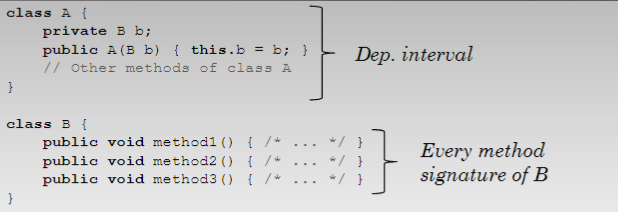
\includegraphics[scale=0.8]{images/asssociazione}
\caption{\textit{Esempio Associazione} \label{fig:ered5}}
\end{figure}

Qual’è lo scopo di dipendenza tra A e B? Siccome stò utilizzando dentro A un oggetto di tipo B, e costruisco A con quel oggetto, l’istanza di B dovrà sempre esistere, quindi ogni metodo di A può usare un istanza di B. Quindi lo scopo è tutta la classe A.

Le firme di tutti i metodi di B possono essere utilizzate in A, quindi è codice condiviso.

Una classe A utilizza una classe B se un oggetto della classe A è in grado di inviare dei messaggi ad un oggetto di classe B oppure se un oggetto di classe A può creare, ricevere o restituire oggetti di classe B.

\subsection{Aggregazione e composizione}
Sono un caso speciale dell’associazione perché un tipo possiede completamente l’altro.

Per esempio le celle di una scacchiera. Perchè sono possedute dalla scacchiera. Una cella non ha senso di esistere al di fuori della scacchiera.

\textbf{L'aggregazione} è una relazione puramente logica. I due oggetti esistono anche se sparisce la relazione. Nell'aggregazione invece tu usi un oggetto come attributo di una nuova classe lo stesso, ma qui non lo vai anche a creare, bensì lo ricevi dall'esterno, ciò significa che l'oggetto aggregante esiste a priori e quindi il ciclo di vita dell'oggetto aggregante è > del ciclo di vita dell'oggetto aggregato.

\textbf{La composizione}, invece, è una relazione più forte. L'oggetto contenuto non può esistere senza il contenitore. Nella composizione tu utilizzi un oggetto come attributo di una nuova classe, ciò comporta che il ciclo di vita dell'oggetto componente ( ex string ) è lo <= del ciclo di vita dell'oggetto composto.

Nella pratica la composizione la tieni quando hai dichiari una reference a string e fai anche la new, l'aggregazione invece quando dichiari solo la reference a string e poi tipo nel costruttore passi un riferimento ad una stringa che è stata creata precedentemente.
\subsubsection{SLOC}

\textbf{SLOC}: source line of code

Quando posso calcolare le linee di codice condivise tra 2 componenti posso formalizzare attraverso una formula matematica, il grado di dipendenza tra i 2 componenti:
\begin{figure}[H]
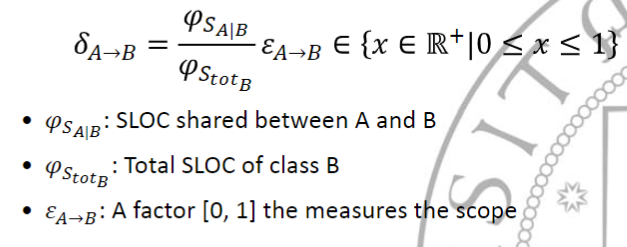
\includegraphics[scale=0.8]{images/SLOC}
\caption{\textit{Definizione di SLOC} \label{fig:sloc}}
\end{figure}
numero linee di codice condivise tra a e b DIVISO il numero di linee complessive di B. Quando ho una dipendenza di tipo Ereditarietà questo limite tende a 1.

Non basta il tipo di dipendenza perché c’è anche lo \textbf{scope}, ovvero il fattore temporale, calcolato in epsilon e cambia a seconda della tipologia di dipendenza. Serve a dar un ordine di importanza alla dipendeze. Per esempio \textbf{l’ereditarietà} ha un epsilon grande in modo da portare l’equazione a 100\%. Più grande è epsion più alta e  la dipendenza. Quindi bisogna scegliere un epsion piccolo.

\textbf{Osservazione}: \textit{Se implemento un’interfaccia oppure se estendo una classe che ha solamente metodi virtuali puri, che tipo di dipendeza c’è?}

L’interfaccia essendo solamente un contratto non è una classe quindi non c’è dipendenza.
  \pagebreak
\section{Observer}
\subsection{Descrizione}
Il pattern Observer, noto anche col nome \textit{Publish-Subscriber}, permette di definire una dipendenza uno a molti fra oggetti, in modo tale che se un oggetto cambia il suo stato interno, ciascuno degli oggetti dipendenti ad esso viene notificato e aggiornato automaticamente.

\subsection{Struttura}
\begin{figure}[H]
\centering
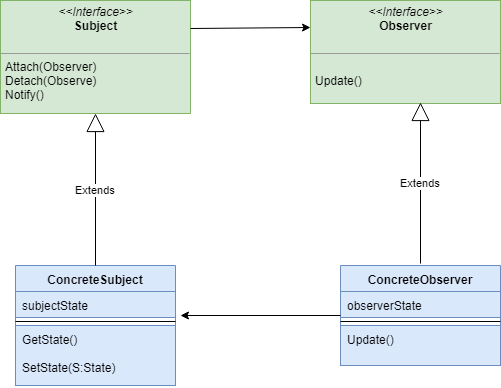
\includegraphics[scale=0.6]{images/observer}
\caption{Struttura observer\label{fig:UC3}}
\end{figure}
\begin{itemize}
	\item \textbf{Subject}
	\begin{itemize}
		\item Il Subject è l'oggetto che notifica li observers;
		\item Il Subject conosce i suoi Observer perchè possiede un riferimento ad essi;
		\item Il metodo \textit{Attach()} serve a sottoscrivere un nuovo observer;
		\item Il metodo \textit{Detach()} serve ad eliminare un observer;
		\item Il metodo \textit{Notify()} sarà implementato dagli observers.
	\end{itemize}
	\item \textbf{ConcreteSubject}
	\begin{itemize}
		\item Quando ConcreteSubject cambia Stato, avverte tutti i ConcreteObserver, attraverso l'invocazione del metodo \textit{Notify()}, ereditato da Subject;
	\end{itemize}
		\item \textbf{Observer}
	\begin{itemize}
		\item Il metodo \textit{Update()} dev'essere implementato dai ConcreteObservers;
	\end{itemize}
	\item \textbf{ConcreteObserver}
	\begin{itemize}
		\item Implementa il metodo \textit{Update()} di Observer;
	\end{itemize}
\end{itemize}

\subsection{Esempio 1}

 Modifica di una o più aree di finestre in risposta alla pressione di un pulsante
\begin{figure}[H]
\centering
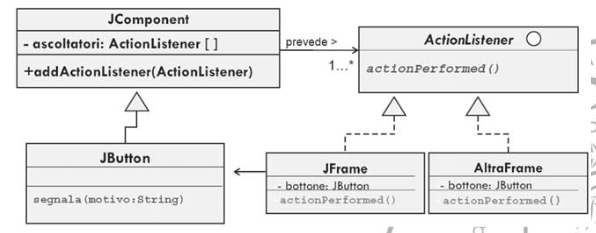
\includegraphics[scale=0.8]{images/esempio1Observer}
\caption{Struttura observer\label{fig:UC3}}
\end{figure}
\begin{itemize}
	\item \textbf{JComponent} agisce da Subject;
	\item \textbf{ActionListener} agisce da Observer;
	\item \textbf{JButton} rappresenta il concreteObserver. È colui che fa scaturire la notifica;
	\item \textbf{JFrame e Altra Frame} rappresentano i concreteObserver;
	\item i 2 concreteObserver hanno un riferimento al concreteSubject ed implementano il metodo \textit{actionPerformed} ereditato da ActionListener;
	\end{itemize}  \pagebreak
\section{Proxy}
\subsection{Descrizione}
Si tratta di un pattern strutturale basato su oggetti che viene utilizzato per accedere ad un’oggetto complesso tramite un oggetto semplice.
Questo pattern può risultare utile se l’oggetto complesso:
\begin{itemize}
\item richiede molte risorse computazionali;
\item richiede molto tempo per caricarsi;
\item è presente su una macchina remota e il traffico di rete determina latenze ed overhead;
\item non definisce delle policy di sicurezze e consente un accesso indiscriminato;
\item non viene mantenuto in cache ma viene rigenerato ad ogni richiesta.
\end{itemize}

\subsection{Applicabilità}
\begin{itemize}
	\item \textbf{Remote Proxy}: rappresentazione locale di un oggetto che si trova in uno spazio di indirizzi differenti. Tipicamente permette di accedere a risorse distribuite sulla rete come se fossero accessibili come oggetto locale;
	\item \textbf{Virtual Proxy}: gestisce la creazione su richiesta di oggetti costosi;
	\item \textbf{Protection Proxy}: controlla l'accesso all'oggetto originale. Questo tipo di proxy si rivela utile quando possono essere definiti diritti di accesso diversi per gli oggetti;
	\item \textbf{Riferimento intelligente}: sostituisce un puntatore puro a un oggetto consentendo l'esecuzione di attività aggiunte quando si accede all'oggetto referenzito;
\end{itemize}

\subsection{Struttura}
\begin{figure}[H]
\centering
\includegraphics[scale=0.6]{images/proxy1}
\caption{Struttura proxy\label{fig:UC3}}
\end{figure}


\begin{itemize}
	\item \textbf{Subject}
	\begin{itemize}
		\item La classe Subject è una classe astratta ed è la classe base del Proxy e del RealSubject;
		\item Definisce i membri che verrano implementati dalle sottoclassi;
	\end{itemize}
	\item \textbf{RealSubject}
	\begin{itemize}
		\item La classe RealSubject è la classe complessa che desideriamo utilizzare in modo efficiente, senza tanto sprecco di risorse;
	\end{itemize}
		\item \textbf{Proxy}
	\begin{itemize}
		\item Gli oggetti Proxy contengono un'istanza privata di un oggetto RealSubject;
		\item Gli oggetti Client eseguono azioni sul proxy che vengono passati all'oggetto RealSubject;
		\item I riusltati dei membri di RealSubject vengono restituiti al client tramite il Proxy.
	\end{itemize}
	
\end{itemize}

Nel diagramma delle classi vediamo come il client dipende solamente dall'interfaccia. Invece dell'oggetto reale, il client potrebbe utilizzare il proxy. Quando l'oggetto proxy viene chiamato fa le sue cose e infine inoltra la chiamata all'oggetto reale.

\subsection{Parole chiavi}
\begin{itemize}
\item \textit{remote proxy}: ambasciatore, governare, remoto, oggetti dislocati nella rete;
\item \textit{virtual proxy}: risorse, locale;
\item \textit{puntatore intelligente}: riferimento, locale;
\end{itemize}

\subsection{Associazione}
\begin{itemize}
\item viene spesso associato con un pattern proxy o adapter o strategy;
\end{itemize}

  \pagebreak

\end{document}
